Although loading and cooling \ce{Be+} ions is fairly straight forward, it is not as clear as how to load \ce{C+} ions into the trap with \ce{Be+} reliably. Early attempts involved using the home-made electron gun to electron dissociate and \ce{CO} gas introduced via leak valve, all possible ionized products of \ce{CO} were detected (\ce{C+}, \ce{O+}, and \ce{CO+}). Even when loading into an empty trap, it was not possible to reliably isolate the \ce{C+} via A-ramping of the trap RF voltage. Prolonged use of the electron gun directly towards the ion trap also caused charging that would slowly dissipate and change the trap parameters. On top of these complications, it would have to work in conjunction with ablation loading \ce{Be+}.

Instead of using two different methods to load the different ion species, ablating both simultaneously was found to be the best method. A sample of \ce{Be} metal was placed on top of a piece of graphite on the target holder so that both samples were in view of the ablation laser. The set up shown in figure \ref{fig: dual ablation} allowed us to separate the ablation laser into two beam with independent alignment and focal planes. The polarization of the laser light is rotated with a half-waveplate, which then enters a polarizing beam splitter (PBS), allowing for tuning of power into either path. The vertically polarized reflected light is reflected again with another PBS and is steered up to the objective lens and then focused into the chamber. The horizontally polarized light transmitted through the first PBS is aligned through an adjustable telescope system. This light is then realigned with the vertically polarized light on the second PBS, co-propagating into the chamber. The "delay stage" for the horizontal light allows for independent focusing and alignment onto the sample.

\todo{draw on figure}
\begin{figure}[H]
	\centering
	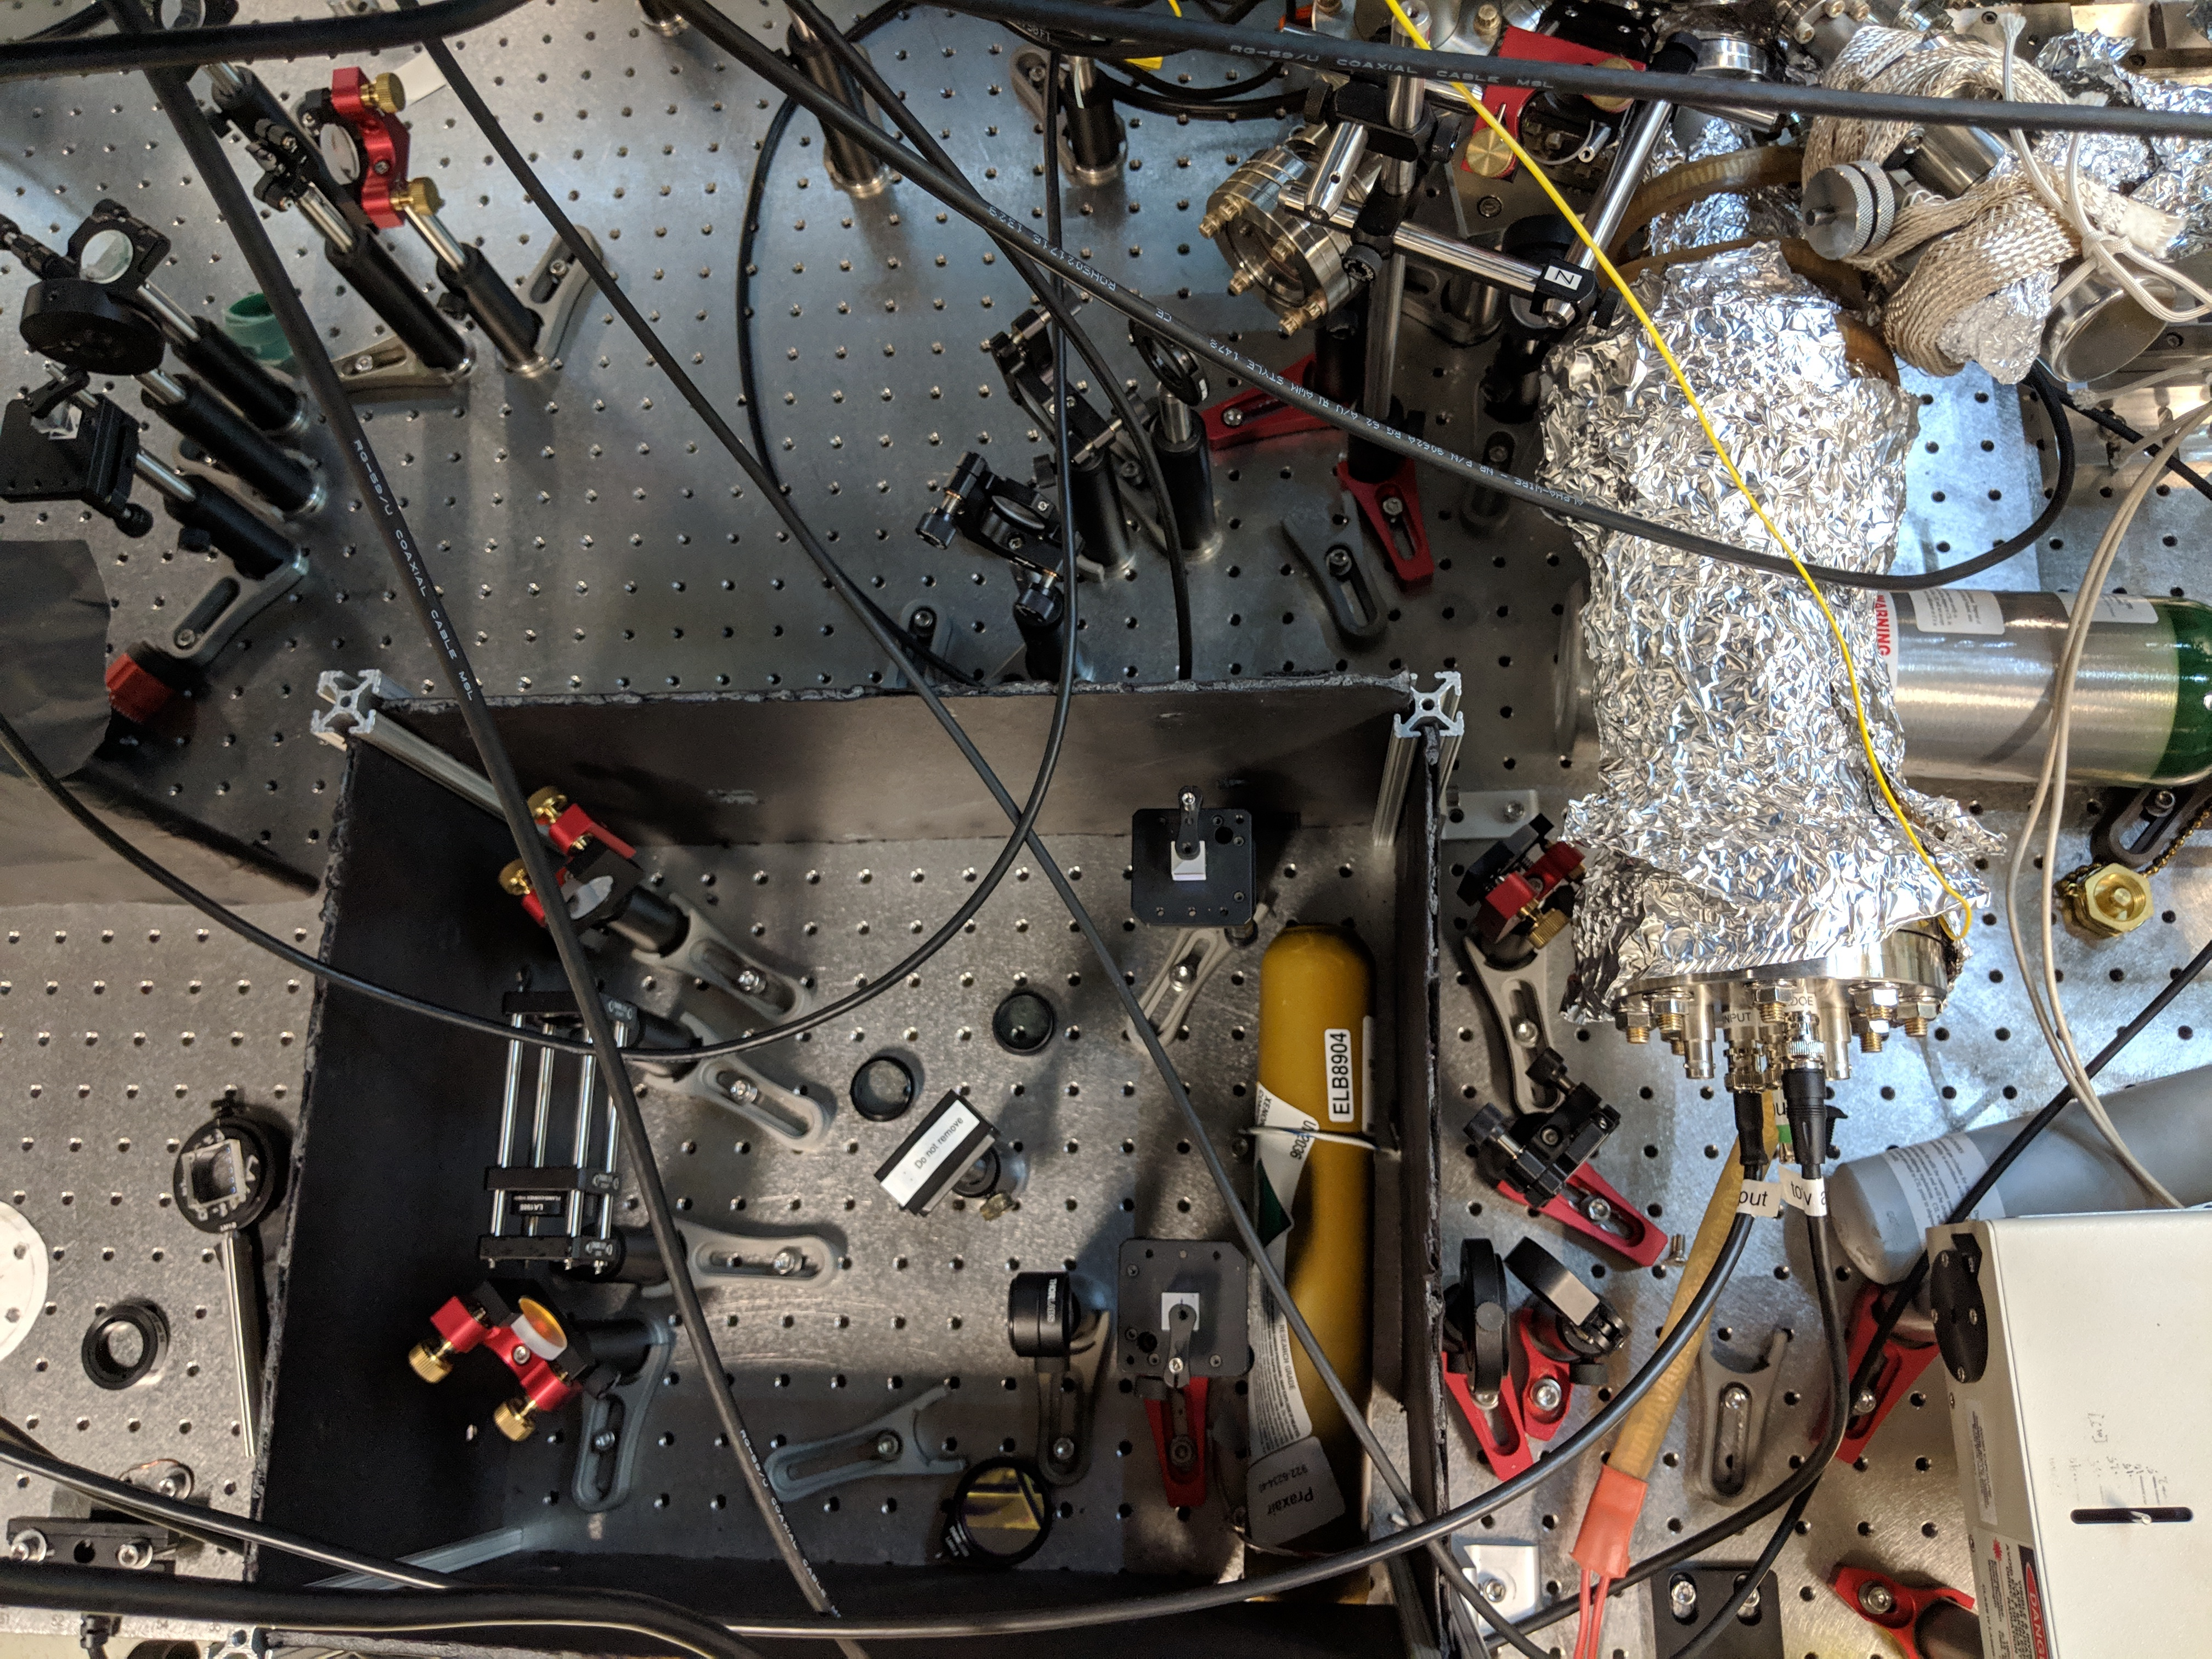
\includegraphics[width=\textwidth]{images/dual_ablation.jpg}
	\caption{Image of the single laser, dual ablation set up. The 1064 nm YAG pulse is split into two paths, and recombined such that they proceed through the same focusing element into the chamber to hit two different targets.}
	\label{fig: dual ablation}
\end{figure}

Blocking one beam allowed for adjustments for the ablation of each species independently. When loading \ce{C+}, we found a strong dependence of the trapped species and the fluence. Lower fluence created not only \ce{C+}, but clusters of, \ce{C2+}, and \ce{C3+} as well. Tight focusing of the beam improves the efficiency of creating only \ce{C+}, but some \ce{Cn+} is still usually produced, which can then be ejected out of the trap with a soft A-ramp.

\begin{figure}[H]
	\centering
	\includegraphics[width=0.8\textwidth]{images/Be_C_TOF.png}
	\caption{TOF trace of simultaneous \ce{Be+} and \ce{C+} ablation loading averaged over 10 shots. A soft A-ramp is applied after loading, ejecting any unintentionally loaded \ce{Cn+} clusters.}
	\label{fig: Be C TOF}
\end{figure}